\documentclass{article}
\usepackage[dblblindworkshop, final]{neurips_2026}
\workshoptitle{The 6th Workshop on Mathematical Reasoning and AI (MATH-AI), NeurIPS 2026}

\usepackage[utf8]{inputenc}
\usepackage[T1]{fontenc}
\usepackage{microtype}
\usepackage{booktabs}
\usepackage{amsmath}
\usepackage{amssymb}
\usepackage{enumitem}
\usepackage{graphicx}
\usepackage{xcolor}
\usepackage{url}
\usepackage{hyperref}
\hypersetup{hidelinks, pdftitle={Detecting and Correcting Reasoning Failures: A Controlled Negative Result for a Residual-Stream Monitor}, pdfauthor={Arnav Kakani, Mrinal Agarwal}}

\graphicspath{{figs/}}

\title{Detecting and Correcting Reasoning Failures:\\
A Controlled Negative Result for a Residual-Stream Monitor}

\author{%
  Arnav Kakani \\
  Emerald High School | Algoverse AI Research\\
  \texttt{arnavkakani@gmail.com} \\
  \And
  Mrinal Agarwal \\
  Emerald High School | Algoverse AI Research\\
  \texttt{smmrinal2009@gmail.com}
}

\begin{document}
\maketitle

\begin{abstract}
Language models often solve math problems with fluent reasoning that still ends in a wrong answer. If the model's internal state signaled the error while the solution was being written, an agent could stop and recompute before committing to it. We test the most direct version of this idea: track how far the hidden state has drifted from where the solution started and, when it drifts too far, roll back a few tokens and prompt the model to recheck its work. We evaluate the monitor by whether the final answer is correct, in the model's intended prompt format, and against controls that isolate what it adds, including a no-intervention baseline and intervening at a random point. Across the evaluated configurations on two open 7B models and two arithmetic benchmarks, the monitor provides no consistent accuracy improvement. In the two configurations with the most incorrect answers, detection AUC is not distinguishable from chance; false-trigger rates reach $98\%$, and monitor-guided intervention shows no recovery advantage over random-position intervention. We also show why letting the model judge its own coherence makes such a method look successful when it is not, and we state the conditions a mid-generation monitor must meet before it can be trusted. \end{abstract}

\section{Introduction}
\label{sec:intro}

A language model can write a math solution that reads fluently but reaches an incorrect answer: an early mistake can propagate through the remaining reasoning \citep{cobbe2021gsm8k, lightman2023verify}. Post-generation checks assess a completed response \citep{kuhn2023semantic, azaria2023internal}. Detecting a potential error during generation could instead allow an intervention before the solution is complete. One possible source of such a signal is the residual stream, the representation each layer reads and updates. Prior work has identified linearly accessible truth-related information in some model representations \citep{marks2023geometry, azaria2023internal}. We test whether drift in the residual stream during generation predicts an incorrect final answer.

We test its simplest version: record the hidden state at the start of each solution, measure how far it moves, and when the distance crosses a threshold, roll back $15$ tokens, insert ``Wait, let me recalculate,'' and let the model continue. \textbf{(RQ1)} Does the drift score predict a wrong final answer? \textbf{(RQ2)} Does acting on it improve final accuracy, compared with the no-intervention baseline and with acting at a random point? We score by the final answer against the reference, not by the model's opinion of its own work; we prompt each model in its intended chat format, which alone raises Qwen2.5-7B's GSM8K accuracy from $0.40$ to $0.90$ and removes the chat-template collapse that raw prompting causes; and we compare every result against the no-intervention baseline, each part of the intervention alone, and a trigger placed at random.

The monitor does not help. Our contributions:
\begin{enumerate}[leftmargin=*,itemsep=1pt,topsep=2pt]
  \item \textbf{A controlled evaluation of residual-stream drift monitoring for arithmetic reasoning} on two open 7B models, two benchmarks, and two distance measures, with three controls.
  \item \textbf{Evidence that neither the signal (RQ1) nor the intervention (RQ2) helps.} Accuracy is unchanged or lower than the no-intervention baseline in five of six settings and within noise in the sixth; the trigger recovers no more errors than a random one; in configurations with more observed errors, the detector ranks them no better than chance and fires on up to $98\%$ of correct solutions.
  \item \textbf{Evidence that a model's judgment of its own coherence cannot replace answer checking}: high coherence ratings on unchanged incorrect answers show that this judge does not reliably measure error correction. We state the bar a mid-generation monitor must clear.
\end{enumerate}

\section{Related work}
\label{sec:related}
Mathematical reasoning in language models is scored by final-answer accuracy on benchmarks such as GSM8K \citep{cobbe2021gsm8k} and SVAMP \citep{patel2021svamp}, and improved by chain-of-thought prompting \citep{wei2022cot}, self-consistency \citep{wang2023selfconsistency}, and step-level verifiers \citep{lightman2023verify}. Self-feedback methods \citep{madaan2023selfrefine, shinn2023reflexion} let the model grade its own output, which is unreliable without an external signal \citep{huang2024cannot} and inherits judge biases \citep{zheng2023judging}. Mechanistic work localizes computation in the residual stream \citep{geva2021transformer, meng2022rome, belrose2023eliciting, bricken2023towards}, finds linear structure for truthfulness \citep{zou2023representation, marks2023geometry, azaria2023internal}, and views generation as a trajectory \citep{elhage2021mathematical, wang2022interpretability}, failure has been framed as gradual drift \citep{spataru2024know, halawi2024overthinking}. Inference-time interventions edit decoding or the cache \citep{chuang2023dola, zhang2024h2o, liu2024snapkv}. Our evaluation focuses on whether residual-stream drift predicts incorrect arithmetic answers and whether interventions guided by that score improve on sampled baselines, greedy continuation controls, and random-position intervention.

\section{Setup}
\label{sec:setup}

We use two open instruction-tuned 7B models, Qwen2.5-7B-Instruct \citep{qwen2024qwen25} (primary) and Mistral-7B-Instruct-v0.1 \citep{jiang2023mistral}, on two grade-school word-problem benchmarks, GSM8K \citep{cobbe2021gsm8k} and SVAMP \citep{patel2021svamp} (SVAMP on the primary model only). With two distance measures this gives six settings, each with its own random-control run. Detection generations are sampled (temperature $0.85$, top-$k$ $50$, up to $400$ tokens; bfloat16 via \texttt{transformer\_lens}, seed $42$); recovery continuations are greedy, up to $256$ tokens; $N{=}100$ problems per setting. An answer counts as correct only if the extracted final number matches the reference. All primary results use reference-answer correctness. A third model, Yi-6B-Chat \citep{ai2024yi}, is excluded for the reason given in Section~\ref{sec:limits}.

\section{Methodology}
\label{sec:method}

\paragraph{Anchor and drift score.}
At layer $\ell$, each generated token $t$ has a residual-stream vector $h_t^{(\ell)}\in\mathbb{R}^d$; we use its direction $\hat h_t = h_t^{(\ell)}/(\lVert h_t^{(\ell)}\rVert_2+\epsilon)$. The first $w_H{=}10$ generated states form a fixed reference anchor for measuring subsequent drift. Each later state receives a drift score. The \emph{L2} score is the squared distance from the current direction to the anchor mean $\bar h$, $D_t = \lVert \hat h_t - \bar h\rVert_2^2$. The \emph{Sinkhorn} score compares sets rather than points: the entropy-regularized 2-Wasserstein distance between the $w_H$ anchor states and the $k{=}5$ most recent states \citep{cuturi2013sinkhorn, feydy2019interpolating}. Each score is converted to a $z$-score against the $5$ states after the anchor (the tare window), and the monitor fires the first time $z$ exceeds a threshold $\tau$. (A Sinkhorn distance between two single vectors is just the squared distance and only the set-to-set form performs any transport.)

\paragraph{What happens on a trigger.}
Generation resumes greedily along four paths on the same problems: \textbf{(A)} no intervention; \textbf{(B)} roll back $r{=}15$ tokens and insert the reset prompt (the full method); \textbf{(C)} insert the prompt without rollback; \textbf{(D)} roll back without the prompt. Clearing the key--value cache changes nothing under greedy decoding, so rollback and prompt insertion are the intervention components.

\paragraph{Random-position control.}
A separate run applies the full intervention at a uniformly random position after the tare window, without looking at the hidden state. It uses the same seed, so its sampled solutions and wrong-answer set are identical to the monitor run's; it fires on every problem, so it controls for where the intervention lands, not how often.

\paragraph{Choosing the operating point, and what we measure.}
The layer (from $\{18,20,22,24,26\}$) and $\tau$ are chosen on held-out data by how well the score separates math from two non-math tasks (Appendix~\ref{app:calib}). For RQ1 we report the AUC of the per-problem maximum $z$-score for predicting a wrong final answer ($0.5$ is a coin flip), with $n_{\text{wrong}}$ (the wrong answers it is estimated from), $n_{\text{genuine}}$ (the triggered wrong answers on which recovery is measured), and the false-trigger rate (the share of correct solutions the monitor fires on). For RQ2 we report final accuracy over all problems and each arm's lift on the genuine-error subset: its wrong$\to$right flips minus its own do-nothing path's.

\section{Results}
\label{sec:results}

\paragraph{RQ1: the drift score does not detectably predict a wrong answer.}
Calibration found no good operating point: one setting met the target only at its boundary and failed validation (Qwen GSM8K Sinkhorn), the rest fell back to the best available separation, and Mistral GSM8K L2 ended at the most permissive threshold ($\tau=2$, fires on $99/100$), hence its $0.98$ false-trigger rate (Appendix~\ref{app:calib}). {Table~\ref{tab:main} reports each setting with the number of wrong answers it contains.} Only the two Mistral settings ($56$ wrong of $100$) give a usable estimate, and both are indistinguishable from a coin flip ($0.514$ and $0.531$; permutation test over $10{,}000$ label shuffles, $p=0.82$ and $0.60$). The $20$ problems used for layer selection are among the $100$ evaluated; on the $80$ disjoint problems the AUCs are $0.517$ (L2, bootstrap 95\% CI $[0.40,0.65]$) and $0.500$ (Sinkhorn, $[0.37,0.62]$), so the overlap does not change the picture (Appendix~\ref{app:calib}). The L2 monitor fires on $48$--$98\%$ of \emph{correct} solutions. The two distance measures agree (AUC $0.53$ vs.\ $0.51$; {accuracy within $0.07$}), so comparing sets instead of points does not help.

\begin{table}[h]
\centering
\small
\caption{Detection and final accuracy ($N=100$ per setting). FT: false-trigger rate. $n_{\text{wrong}}/n_{\text{gen}}$: triggered baseline errors. S: sampled baseline. C: prompt only. B: full intervention. Random: random position intervention.}\label{tab:main}
\begin{tabular}{llccccccccc}
\toprule
& & & \multicolumn{4}{c}{\bf Detection} & \multicolumn{4}{c}{\bf Final accuracy} \\
\cmidrule(lr){4-7}\cmidrule(lr){8-11}
\bf Model & \bf Dataset & \bf Metric & \bf AUC & $\boldsymbol{n_{\text{wrong}}}$ & $\boldsymbol{n_{\text{gen}}}$ & \bf FT & \bf S & \bf C & \bf B & \bf Random \\
\midrule
Qwen2.5-7B & GSM8K & Sinkhorn & 0.62 & 10 & 2  & 0.17 & 0.90 & 0.89 & 0.89 & 0.92 \\
Qwen2.5-7B & GSM8K & L2       & 0.46 & 10 & 5  & 0.48 & 0.90 & 0.87 & 0.87 & 0.92 \\
Qwen2.5-7B & SVAMP & Sinkhorn & 0.67 & 7 & 6  & 0.89 & 0.93 & 0.91 & 0.93 & 0.91 \\
Qwen2.5-7B & SVAMP & L2       & 0.55 & 7 & 6  & 0.96 & 0.93 & 0.93 & 0.91 & 0.91 \\
Mistral-7B & GSM8K & Sinkhorn & \bf 0.51 & \bf 56 & 35 & 0.68 & 0.44 & 0.46 & 0.46 & 0.37 \\
Mistral-7B & GSM8K & L2       & \bf 0.53 & \bf 56 & 56 & 0.98 & 0.44 & 0.44 & 0.39 & 0.37 \\
\bottomrule
\end{tabular}
\end{table}

\paragraph{The failures are real arithmetic errors, not formatting collapse.}
Without the chat template, most failures are template collapse (the model emits formatting tokens and stops reasoning); with it, classifying every triggered wrong answer by its generated text, no setting contains one. On Mistral, $50/56$ (L2) and $29/35$ (Sinkhorn) failures are complete solutions with a wrong answer, the rest never reach an answer; on Qwen, $15/19$. This classification reads the greedy continuation from the trigger point (the sampled text was not stored), and $6$ of the $50$ and $5$ of the $29$ continuations are in fact correct; it characterizes the failure mode the monitor acts on, not the original sampled errors themselves (Appendix~\ref{app:typ}). The signal is not empty: on Mistral Sinkhorn it separates math from summarization by $z_{\text{gap}}=5.10$ while ranking correct against incorrect math at $0.514$; it tracks what task the model is doing, not whether it is doing it right.

\paragraph{RQ2: acting on the score does not detectably beat doing nothing or a random trigger.}
Table~\ref{tab:main} reports final accuracy over all $100$ problems in each setting, which is the number an agent would actually see. Two reference points are involved and must be kept apart. The \emph{sampled baseline} is the accuracy of the original sampled solution with no intervention at all ($0.44$ on Mistral GSM8K, $0.90$--$0.93$ on Qwen); this is the Table~\ref{tab:main} column labeled S. The \emph{greedy continuation control}, path A in Section~\ref{sec:method}, restarts greedy decoding from the trigger point with no rollback and no prompt; because it is a fresh decode, it fixes some errors on its own, and on Mistral it reaches $0.41$ (L2), $0.45$ (Sinkhorn) and $0.40$ (random run) over all $100$ problems. Against the sampled baseline, the full method is unchanged or lower in five of six settings and higher by $0.02$ in the sixth, and every Mistral Wilson $95\%$ interval contains the $0.44$ baseline (Appendix~\ref{app:did}); on both Qwen GSM8K settings the random-position trigger is nominally the best path ($0.92$ vs.\ $0.90$), a difference of two problems. Against its own continuation control, the paired full-minus-control difference, bootstrapped over problems, is $-0.02$ $[-0.11,+0.07]$ on L2, $+0.01$ $[-0.06,+0.08]$ on Sinkhorn and $-0.03$ $[-0.11,+0.05]$ on the random run; each interval straddles zero. The intervention also has a cost the headline hides: the full method turns $14$, $5$ and $13$ initially correct answers wrong in those three runs, comparable to the number it fixes ($9$, $7$ and $6$).

The recovery question is narrower: among problems the sampled baseline got wrong, how many does each path turn right, and does the monitor's choice of \emph{where} to intervene add anything over a random position? We report lift, each arm's wrong$\to$right flips minus its own continuation control's, because the control already repairs some errors. On Mistral L2 the full method flips $9$ of $56$ wrong answers against the control's $6$ (lift $+3$), and the random trigger flips $6$ against $3$ (also $+3$). On Sinkhorn the monitor fires on only $35$ of the $56$ errors, so its $+2$ against random's $+3$ over all $56$ compares two policies that intervene on different problems; restricted to the $35$ problems both intervene on, the monitor's lift is $+2$ and random's is $-1$, a matched-timing comparison on too few cases to separate them (Appendix~\ref{app:did}). Trigger positions are consistent with this: on Mistral L2 the median trigger is token $17$, immediately after the $10$-token anchor and $5$-token tare window and before any arithmetic has appeared, so the ``recovery'' is a restart of the solution rather than a correction of a located error; in the other settings the median trigger falls between tokens $25$ and $69$ (Appendix~\ref{app:trig}). Equal lift does not prove equivalence, but using the hidden state recovers no detectably more errors than a random point, in line with evidence that models do not correct their own reasoning without outside feedback \citep{huang2024cannot}. Sweeping $\tau$ on Qwen GSM8K L2, accuracy returns to the $0.90$ baseline once the threshold is high enough that the monitor fires on at most $45\%$ of problems (Appendix~\ref{app:sweep}).

\paragraph{A model judging its own coherence cannot score recovery.}
Recovery is often scored by asking the model whether its output stayed coherent. We scored our paths that way, a ``sound''/``drifted'' verdict from the model under test without the reference (Appendix~\ref{app:judge}, Figure~\ref{fig:judge}). On Mistral it reports $82$--$95\%$ ``recovery'' on paths whose real wrong$\to$right rate is $0.05$--$0.20$, and across all six settings it scores \emph{doing nothing} at $0.76$--$0.91$, including $0.91$ on Mistral GSM8K L2 where accuracy is $0.44$. The score does not track accuracy across models ($0.91$ for a $0.44$-accurate model, $0.85$ for a $0.90$-accurate one) and rates Qwen's intervened paths below its baseline ($0.55$--$0.72$ vs.\ $0.76$--$0.85$). The judge rate is computed over the cases with a parseable verdict ($55$ of $99$ triggered cases for path A on Mistral L2) and the correction rate over the $56$ originally wrong cases; the run did not store per-case verdicts, so the two cannot be joined on a common set, and the comparison is between population rates, not paired outcomes. A judge that calls doing nothing a success cannot substitute for checking the answer.

\section{Limitations}
\label{sec:limits}

Our evidence covers short arithmetic reasoning on instruction-tuned models without a long-reasoning mode. Qwen2.5-7B provides four settings, but at $0.90$--$0.93$ accuracy it yields only seven to ten wrong answers per setting, resulting in wide AUC confidence intervals; the configurations with the most observed errors are therefore both Mistral-7B on GSM8K. A test that cannot reject chance does not prove chance, so our claim is \emph{no detectable signal at this sample size}. Mistral's low baseline is genuine ($50/56$ failures are complete solutions with a wrong answer); Yi-6B-Chat (baseline $0.04$) is excluded because $64/80$ of its failures never state an answer. The $256$-token recovery budget roughly doubles truncation under the intervention on Mistral ($9/99$ to $18/99$). This difference may disadvantage the intervention and limits conclusions about its effectiveness with longer recovery budgets. The layer and threshold were chosen by how well the score separates math from non-math tasks, not correct from incorrect solutions; the threshold-free AUC does not depend on $\tau$, but the layer does, and correctness-based layer selection and a supervised probe on the same activations were not run. Both are the first things to try, together with a task on which the stronger model still fails.

These results do not rule out internal signals of arithmetic failure. They show that the drift scores and interventions evaluated here provide no reliable detection or correction benefit under the tested conditions, and they set the bar such a monitor must clear: (i) score by the final answer against the reference, in the model's own prompt format; (ii) beat doing nothing on the full task; (iii) beat a random-position trigger on the genuine-error subset, as lift over each arm's own continuation control; (iv) rank failures above chance where there are enough failures to estimate it; and (v) still work after removing each component. Since capable small models are close to ceiling on GSM8K, this kind of evaluation should use a task they still fail. The monitor studied here clears none.


\newpage

\bibliographystyle{unsrtnat}
\bibliography{references}

\newpage

\appendix
\section{Code availability}
\label{app:code}
The code, run artifacts, and figure scripts are available at
\url{https://github.com/ArnavKakani/DCRF}.

\section{Layer and threshold selection}
\label{app:calib}
The layer is chosen by $z_{\text{gap}} = \overline{\max z}_{\text{target}} -
\overline{\max z}_{\text{control}}$ over $20$ target and $2\times20$ control problems
(CNN/DailyMail, MBPP), one rollout, and the threshold on a parity split of those traces.
Selected operating points are in Table~\ref{tab:calib}. The $20$ layer-selection problems are problems $0$--$19$ of the evaluated $100$; detection AUC on the $80$ remaining problems is $0.517$ for L2 ($43$ wrong; bootstrap 95\% CI $[0.40,0.65]$) and $0.500$ for Sinkhorn ($[0.37,0.62]$).

\begin{table}[h]
\centering\small
\caption{Selected operating points. TPR/FPR are trigger rates on reasoning vs.\ control
tasks at the selected $\tau$ (task separation, not error separation). Five of six cells miss the target and fall back to best separation; the sixth meets it only at the boundary. Bootstrap 95\% AUC intervals for the Qwen cells span $0.27$--$0.93$.}
\label{tab:calib}
\begin{tabular}{llcccc}
\toprule
\bf Cell & \bf Layer ($z_{\text{gap}}$) & $\boldsymbol\tau$ & \bf fit TPR & \bf fit FPR & \bf met target \\
\midrule
Qwen GSM8K L2 & 18 (0.016) & 6.0 & 0.70 & 0.60 & no \\
Qwen GSM8K Sinkhorn & 22 & 15.0 & 0.60 & 0.20 & borderline \\
Qwen SVAMP L2 & 26 & 4.0 & 1.00 & 0.80 & no \\
Qwen SVAMP Sinkhorn & 26 & 6.0 & 1.00 & 0.65 & no \\
Mistral GSM8K L2 & 18 (0.578) & 2.0 & 1.00 & 0.90 & no \\
Mistral GSM8K Sinkhorn & 20 (5.10) & 6.0 & 1.00 & 0.45 & no \\
\bottomrule
\end{tabular}
\end{table}

\section{Threshold sweep and seed robustness}
\label{app:sweep}
Qwen GSM8K L2, $20$ problems per threshold: final accuracy $0.75$ ($\tau{=}2$), $0.70$
($4$), $0.75$ ($6$), $0.90$ ($8$, $10$, $12.5$, $15$); trigger rate falls from $1.00$ to
$0.10$ over the same grid (Figure~\ref{fig:sweep}). Trigger rate over five seeds ($30$ problems each) is
$0.57\pm0.04$.
\begin{figure}[h]
\centering
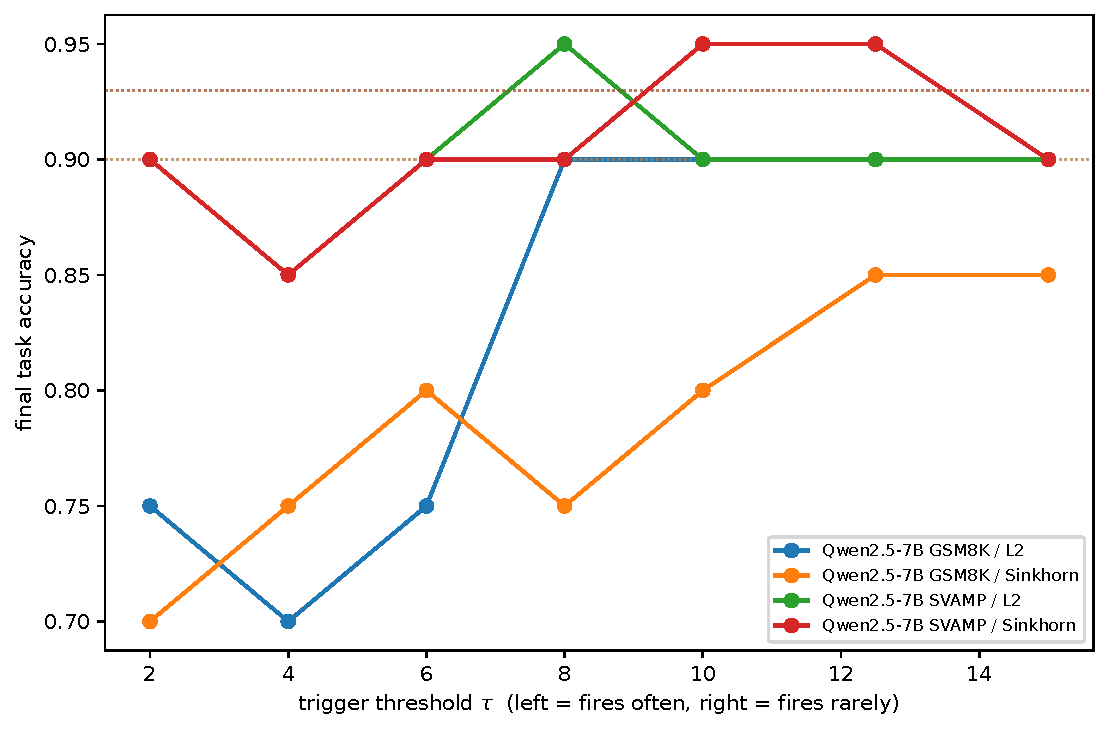
\includegraphics[width=0.6\linewidth]{fig_intervention_cost}
\caption{Final accuracy vs.\ trigger threshold on Qwen GSM8K L2 ($n{=}20$ per point). Accuracy returns to the $0.90$ baseline only once the detector stops firing ($\tau\ge 8$).}
\label{fig:sweep}
\end{figure}

\section{Failure typology}
\label{app:typ}
Triggered baseline failures classified on the generated text with the prompt stripped and
the model's end-of-turn token removed. ``Wrong answer'': a well-formed solution stating a
wrong final answer. ``No answer'': looping or cut off by the budget. The text classified is path A, the greedy continuation from the trigger point; the original sampled generation was not stored. Of the Mistral ``wrong answer'' continuations, $6/50$ (L2) and $5/29$ (Sinkhorn) are correct under the extractor. Table~\ref{tab:typ} and Figure~\ref{fig:typ} give the counts.
\begin{table}[h]
\centering\small
\caption{Typology of triggered baseline failures, classified on the generated text with the
prompt stripped and the end-of-turn token removed. No cell contains a template collapse; Mistral's failures are overwhelmingly wrong answers, Yi's are non-completion.}
\label{tab:typ}
\begin{tabular}{lcccc}
\toprule
\bf Cell & \bf $n$ & \bf Wrong answer & \bf No answer & \bf Template collapse \\
\midrule
Qwen GSM8K L2 & 5 & 3 & 2 & 0 \\
Qwen GSM8K Sinkhorn & 2 & 1 & 1 & 0 \\
Qwen SVAMP L2 & 6 & 6 & 0 & 0 \\
Qwen SVAMP Sinkhorn & 6 & 5 & 1 & 0 \\
Mistral GSM8K L2 & 56 & 50 & 6 & 0 \\
Mistral GSM8K Sinkhorn & 35 & 29 & 6 & 0 \\
Yi GSM8K L2 (excluded) & 80 & 16 & 64 & 0 \\
\bottomrule
\end{tabular}
\end{table}
\begin{figure}[h]
\centering
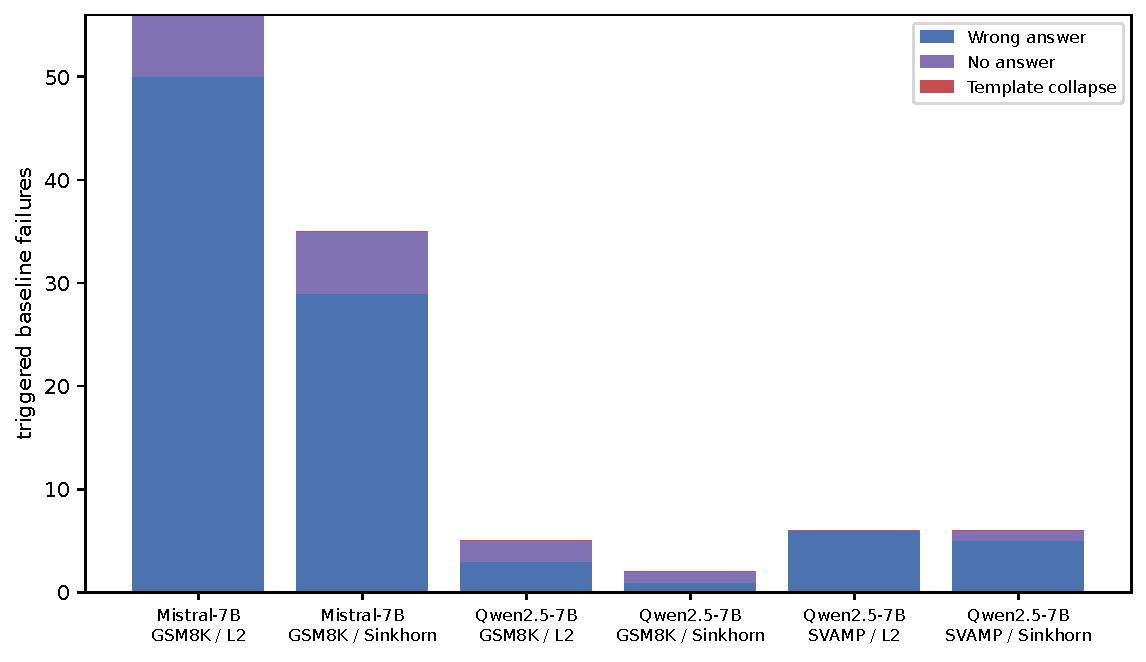
\includegraphics[width=0.75\linewidth]{fig_typology}
\caption{Typology of triggered baseline failures, as in Table~\ref{tab:typ}: wrong answers dominate on Qwen and Mistral, non-completion on Yi, template collapse nowhere.}
\label{fig:typ}
\end{figure}

\section{Coherence judge vs.\ answer correctness}
\label{app:judge}
\begin{figure}[h]
\centering
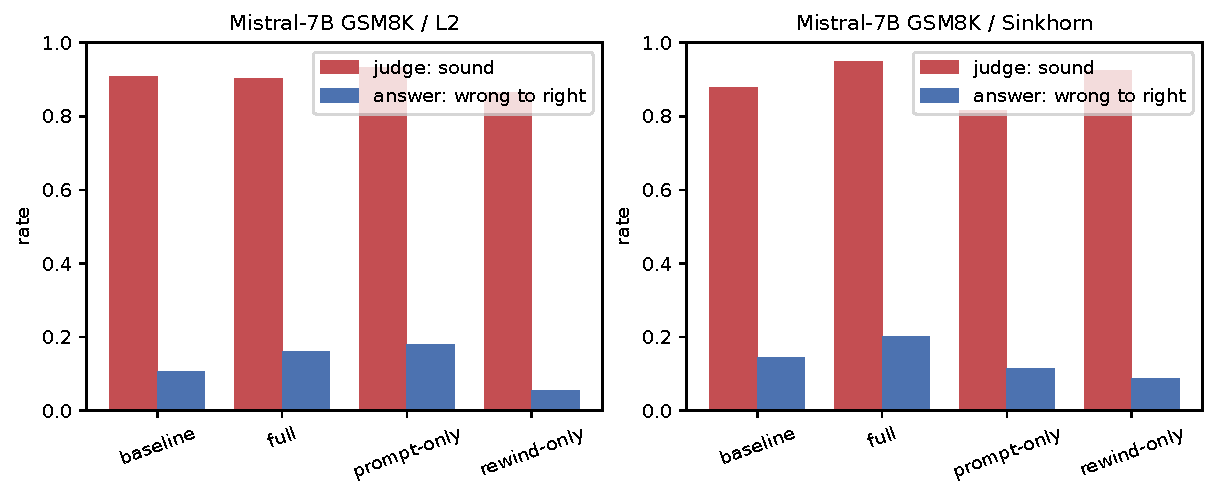
\includegraphics[width=0.5\linewidth]{fig_judge_artifact}
\caption{A model judging its own coherence vs.\ the true answer on the same generations (Mistral). The
judge awards $0.82$--$0.95$ ``recovery'' to every path, including doing nothing, while the real wrong$\to$right rate is $0.05$--$0.20$. Judge rates are over cases with a parseable verdict (Mistral L2: A $55$, B $52$, C $44$, D $59$ of $99$ triggered); correction rates are over the $56$ originally wrong cases. Per-case verdicts were not stored, so the two populations cannot be joined.}
\label{fig:judge}
\end{figure}

\section{Matched recovery comparison}
\label{app:did}
The random-control run reproduces the detector run's sampled trajectories (identical
seed), so the baseline-wrong sets coincide exactly (Mistral: the same $56$ problems).
Wrong$\to$right flips on that set are in Table~\ref{tab:did}:
\begin{table}[h]
\centering
\small
\setlength{\tabcolsep}{3pt}
\caption{Wrong$\to$right flips per path on the shared baseline-wrong set. Wilson 95\% intervals on Mistral final accuracy: full L2 $[0.30,0.49]$, full Sinkhorn $[0.37,0.56]$, random $[0.28,0.47]$, all containing the $0.44$ baseline. A is the greedy continuation control, not the sampled baseline. Lift $B{-}A$: detector $+3$ vs.\ random $+3$ on Mistral L2; $+2$ vs.\ $+3$ on
Sinkhorn over all $56$ errors (a policy comparison, since Sinkhorn triggers on $35$ of them); on the $35$ shared cases, monitor A $5$, B $7$ ($+2$) vs.\ random A $3$, B $2$ ($-1$). Paired full-minus-control accuracy differences over all $100$: $-0.02$ $[-0.11,+0.07]$ (L2), $+0.01$ $[-0.06,+0.08]$ (Sinkhorn), $-0.03$ $[-0.11,+0.05]$ (random). Truncation at the $256$-token
recovery budget on Mistral L2: A $9/99$, B $18/99$, C $16/99$, D $16/99$; random run A
$4/100$, B $8/100$.}
\label{tab:did}
\setlength{\tabcolsep}{4pt}
\begin{tabular}{@{}lcccccc@{}}
\toprule
\textbf{Cell} & \textbf{A} & \textbf{B} & \textbf{C}
& \textbf{D} & \multicolumn{2}{c}{\textbf{Random}} \\
\cmidrule(lr){6-7}
& Control & Full & Prompt & Rollback & A & B \\
\midrule
Mistral GSM8K L2 ($n{=}56$)
& 6 & 9 & 10 & 3 & 3 & 6 \\
Mistral GSM8K Sinkhorn ($n{=}35$)
& 5 & 7 & 4 & 3 & (3/56) & (6/56) \\
Qwen GSM8K L2 ($n{=}5$)
& 1 & 1 & 1 & 1 & (3/10) & (3/10) \\
\bottomrule
\end{tabular}
\end{table}

\section{Trigger positions}
\label{app:trig}
Figure~\ref{fig:trig} shows where the monitor fires in each setting. The anchor ($10$ tokens) and tare window ($5$ tokens) end at token $15$. Median trigger index: Mistral GSM8K L2 $17$ ($65$ of $99$ triggers at or before token $20$; $19$ at exactly $15$), Mistral GSM8K Sinkhorn $31$, Qwen GSM8K L2 $67$, Qwen GSM8K Sinkhorn $69$, Qwen SVAMP L2 $25$, Qwen SVAMP Sinkhorn $47$.

\begin{figure}[h]
\centering
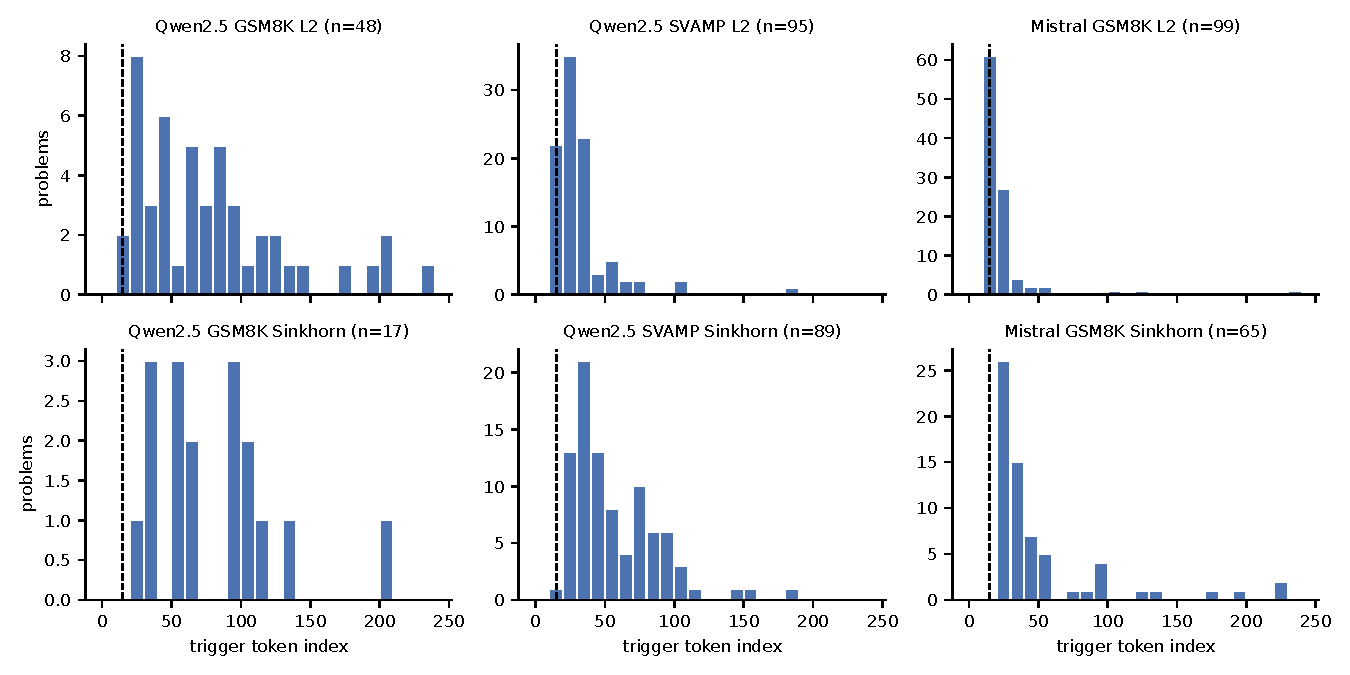
\includegraphics[width=0.9\linewidth]{fig_trigger_positions}
\caption{Trigger token index by setting. The dashed line marks index $15$, the reported boundary of the anchor and tare windows. On Mistral GSM8K L2, $65$ of $99$ triggers occur at or before index $20$; median trigger indices in the other settings range from $25$ to $69$. The histogram measures trigger position, not whether an arithmetic operation has occurred.}
\label{fig:trig}
\end{figure}

\section{Before and after examples}
\label{app:examples}
Two genuine-error cases from Mistral-7B GSM8K L2 (prompt stripped; generated text verbatim). In both, the detector fires at token $17$--$18$, immediately after the tare window and before any arithmetic has been performed, so the ``recovery'' is a fresh derivation from the start of the solution. That is why a random position does as well.

\paragraph{Recovered (gold $44$; spike at token $17$).}
\emph{Q:} Gene is sewing a quilt out of old souvenir t-shirts. He has one shirt from each vacation he has been on. Every shirt is its own quilt block. Each row is made of blocks from a different year of vacations. He goes on four vacations a year and has been vacationing since he was 23 years old. He is now 34. How many quilt blocks does he have in total?

\emph{Do nothing (A), wrong:} ``\ldots in 34 years (the age he is now), he would have gone on a total of 34 x 4 = 136 vacations. \ldots The answer is 136.''

\emph{Full method (B), right:} ``Let' \textbackslash n Wait, let me recalculate this step to be sure: 1. From 23 to 34, Gene has been on vacation for 11 years. 2. \ldots 11 x 4 = 44 vacations. \ldots The answer is 44.''

\paragraph{Not recovered (gold $14$; spike at token $18$).}
\emph{Q:} Raymond and Samantha are cousins. Raymond was born 6 years before Samantha. Raymond had a son at the age of 23. If Samantha is now 31, how many years ago was Raymond's son born?

\emph{Do nothing (A), wrong:} ``\ldots Raymond had a son at the age of 23. So, Raymond's son was born 23 years ago. The answer is 23 years ago.''

\emph{Full method (B), still wrong:} ``Let's \textbackslash n Wait, let me recalculate this step to be sure: 1. Raymond was born 6 years before Samantha. 2. Samantha is now 31. 3. Therefore, Raymond was born 31 - 6 = 25 years ago. The answer is 25.''

\section{Ethics statement and reproducibility}
\label{app:ethics}
This work uses public benchmarks and open models and involves no human subjects. It reports a negative result with its uncertainty stated, and is intended to support careful reporting of inference-time reliability claims for mathematical agents; we foresee no negative impact from a negative result on public benchmarks.

Each run writes a self-contained directory with a manifest (model, dataset, full configuration snapshot, per-stage status) and all intermediate artifacts (trajectories, ablation paths, labels, judge outputs). Every table and figure regenerates from those artifacts without re-running the models; the code and artifacts are at \url{https://github.com/ArnavKakani/DCRF} (Appendix~\ref{app:code}). One known limitation: the answer extractor disagrees with a strict ``answer is $N$'' parse on $29$ of $3{,}524$ recovery texts, most of them negative dollar amounts written as \texttt{-\$N}; none of the correctness outcomes we checked is affected.

All runs executed on single NVIDIA H100 and A100 instances rented from Lambda, one 7B model in \texttt{bfloat16} at a time, over roughly $19$ wall-clock hours for the eleven runs (June 24--25, 2026). Assets: GSM8K and SVAMP (MIT license), Qwen2.5-7B-Instruct and Mistral-7B-Instruct-v0.1 (Apache-2.0), Yi-6B-Chat (Yi model license), \texttt{transformer\_lens} and \texttt{geomloss} (MIT).

\clearpage
\section*{NeurIPS Paper Checklist}

\begin{enumerate}

\item {\bf Claims}
    \item[] Question: Do the main claims made in the abstract and introduction accurately reflect the paper's contributions and scope?
    \item[] Answer: \answerYes{}
    \item[] Justification: The abstract and introduction claim a controlled negative result on six model$\times$dataset$\times$metric configurations, a matched random-control comparison, chance-indistinguishable detection where powered, and the coherence-judge comparison; Sections~3--5 and Appendix~\ref{app:judge} report exactly these, with scope limited to short arithmetic reasoning.
    \item[] Guidelines:
    \begin{itemize}
        \item The answer \answerNA{} means that the abstract and introduction do not include the claims made in the paper.
        \item The abstract and/or introduction should clearly state the claims made, including the contributions made in the paper and important assumptions and limitations. A \answerNo{} or \answerNA{} answer to this question will not be perceived well by the reviewers. 
        \item The claims made should match theoretical and experimental results, and reflect how much the results can be expected to generalize to other settings. 
        \item It is fine to include aspirational goals as motivation as long as it is clear that these goals are not attained by the paper. 
    \end{itemize}

\item {\bf Limitations}
    \item[] Question: Does the paper discuss the limitations of the work performed by the authors?
    \item[] Answer: \answerYes{}
    \item[] Justification: Section~\ref{sec:limits} states the single powered model, the inability of a permutation test to prove exact chance, the recovery-budget truncation confound, the $n{=}20$ threshold sweep, the position (not rate-matched) random control, and the exclusion of Yi-6B-Chat.
    \item[] Guidelines:
    \begin{itemize}
        \item The answer \answerNA{} means that the paper has no limitation while the answer \answerNo{} means that the paper has limitations, but those are not discussed in the paper. 
        \item The authors are encouraged to create a separate ``Limitations'' section in their paper.
        \item The paper should point out any strong assumptions and how robust the results are to violations of these assumptions (e.g., independence assumptions, noiseless settings, model well-specification, asymptotic approximations only holding locally). The authors should reflect on how these assumptions might be violated in practice and what the implications would be.
        \item The authors should reflect on the scope of the claims made, e.g., if the approach was only tested on a few datasets or with a few runs. In general, empirical results often depend on implicit assumptions, which should be articulated.
        \item The authors should reflect on the factors that influence the performance of the approach. For example, a facial recognition algorithm may perform poorly when image resolution is low or images are taken in low lighting. Or a speech-to-text system might not be used reliably to provide closed captions for online lectures because it fails to handle technical jargon.
        \item The authors should discuss the computational efficiency of the proposed algorithms and how they scale with dataset size.
        \item If applicable, the authors should discuss possible limitations of their approach to address problems of privacy and fairness.
        \item While the authors might fear that complete honesty about limitations might be used by reviewers as grounds for rejection, a worse outcome might be that reviewers discover limitations that aren't acknowledged in the paper. The authors should use their best judgment and recognize that individual actions in favor of transparency play an important role in developing norms that preserve the integrity of the community. Reviewers will be specifically instructed to not penalize honesty concerning limitations.
    \end{itemize}

\item {\bf Theory assumptions and proofs}
    \item[] Question: For each theoretical result, does the paper provide the full set of assumptions and a complete (and correct) proof?
    \item[] Answer: \answerYes{}
    \item[] Justification: The one analytic statement (optimal transport between two single normalized vectors reduces to the ground cost) is stated with its assumption in Section~\ref{sec:method}; it follows directly from the definition of a coupling between point masses.
    \item[] Guidelines:
    \begin{itemize}
        \item The answer \answerNA{} means that the paper does not include theoretical results. 
        \item All the theorems, formulas, and proofs in the paper should be numbered and cross-referenced.
        \item All assumptions should be clearly stated or referenced in the statement of any theorems.
        \item The proofs can either appear in the main paper or the supplemental material, but if they appear in the supplemental material, the authors are encouraged to provide a short proof sketch to provide intuition. 
        \item Inversely, any informal proof provided in the core of the paper should be complemented by formal proofs provided in appendix or supplemental material.
        \item Theorems and Lemmas that the proof relies upon should be properly referenced. 
    \end{itemize}

    \item {\bf Experimental result reproducibility}
    \item[] Question: Does the paper fully disclose all the information needed to reproduce the main experimental results of the paper to the extent that it affects the main claims and/or conclusions of the paper (regardless of whether the code and data are provided or not)?
    \item[] Answer: \answerYes{}
    \item[] Justification: Sections~\ref{sec:setup}--\ref{sec:method} and Appendices~\ref{app:calib}--\ref{app:examples} give models, datasets, sample sizes, seed, decoding parameters, window sizes, rollback length, reset text, layer band, threshold grid, calibration rule, and the selected operating points per cell.
    \item[] Guidelines:
    \begin{itemize}
        \item The answer \answerNA{} means that the paper does not include experiments.
        \item If the paper includes experiments, a \answerNo{} answer to this question will not be perceived well by the reviewers: Making the paper reproducible is important, regardless of whether the code and data are provided or not.
        \item If the contribution is a dataset and\slash or model, the authors should describe the steps taken to make their results reproducible or verifiable. 
        \item Depending on the contribution, reproducibility can be accomplished in various ways. For example, if the contribution is a novel architecture, describing the architecture fully might suffice, or if the contribution is a specific model and empirical evaluation, it may be necessary to either make it possible for others to replicate the model with the same dataset, or provide access to the model. In general. releasing code and data is often one good way to accomplish this, but reproducibility can also be provided via detailed instructions for how to replicate the results, access to a hosted model (e.g., in the case of a large language model), releasing of a model checkpoint, or other means that are appropriate to the research performed.
        \item While NeurIPS does not require releasing code, the conference does require all submissions to provide some reasonable avenue for reproducibility, which may depend on the nature of the contribution. For example
        \begin{enumerate}
            \item If the contribution is primarily a new algorithm, the paper should make it clear how to reproduce that algorithm.
            \item If the contribution is primarily a new model architecture, the paper should describe the architecture clearly and fully.
            \item If the contribution is a new model (e.g., a large language model), then there should either be a way to access this model for reproducing the results or a way to reproduce the model (e.g., with an open-source dataset or instructions for how to construct the dataset).
            \item We recognize that reproducibility may be tricky in some cases, in which case authors are welcome to describe the particular way they provide for reproducibility. In the case of closed-source models, it may be that access to the model is limited in some way (e.g., to registered users), but it should be possible for other researchers to have some path to reproducing or verifying the results.
        \end{enumerate}
    \end{itemize}


\item {\bf Open access to data and code}
    \item[] Question: Does the paper provide open access to the data and code, with sufficient instructions to faithfully reproduce the main experimental results, as described in supplemental material?
    \item[] Answer: \answerYes{}
    \item[] Justification: A repository is linked at submission through github with documented pipelines (Appendix~\ref{app:code}). 
    \item[] Guidelines:
    \begin{itemize}
        \item The answer \answerNA{} means that paper does not include experiments requiring code.
        \item Please see the NeurIPS code and data submission guidelines (\url{https://neurips.cc/public/guides/CodeSubmissionPolicy}) for more details.
        \item While we encourage the release of code and data, we understand that this might not be possible, so \answerNo{} is an acceptable answer. Papers cannot be rejected simply for not including code, unless this is central to the contribution (e.g., for a new open-source benchmark).
        \item The instructions should contain the exact command and environment needed to run to reproduce the results. See the NeurIPS code and data submission guidelines (\url{https://neurips.cc/public/guides/CodeSubmissionPolicy}) for more details.
        \item The authors should provide instructions on data access and preparation, including how to access the raw data, preprocessed data, intermediate data, and generated data, etc.
        \item The authors should provide scripts to reproduce all experimental results for the new proposed method and baselines. If only a subset of experiments are reproducible, they should state which ones are omitted from the script and why.
        \item At submission time, to preserve anonymity, the authors should release anonymized versions (if applicable).
        \item Providing as much information as possible in supplemental material (appended to the paper) is recommended, but including URLs to data and code is permitted.
    \end{itemize}


\item {\bf Experimental setting/details}
    \item[] Question: Does the paper specify all the training and test details (e.g., data splits, hyperparameters, how they were chosen, type of optimizer) necessary to understand the results?
    \item[] Answer: \answerYes{}
    \item[] Justification: No training is performed. Test splits, prompt template, sampling and greedy decoding settings, anchor/tare/recent windows, and the held-out threshold-calibration procedure are given in Sections~\ref{sec:setup}--\ref{sec:method} and Appendix~\ref{app:calib}.
    \item[] Guidelines:
    \begin{itemize}
        \item The answer \answerNA{} means that the paper does not include experiments.
        \item The experimental setting should be presented in the core of the paper to a level of detail that is necessary to appreciate the results and make sense of them.
        \item The full details can be provided either with the code, in appendix, or as supplemental material.
    \end{itemize}

\item {\bf Experiment statistical significance}
    \item[] Question: Does the paper report error bars suitably and correctly defined or other appropriate information about the statistical significance of the experiments?
    \item[] Answer: \answerYes{}
    \item[] Justification: Detection AUCs carry the number of genuine failures and two-sided permutation $p$-values; final accuracies carry Wilson 95\% intervals; recovery is compared as matched lift on identical failure sets; trigger-rate variability over five seeds is reported in Appendix~\ref{app:sweep}.
    \item[] Guidelines:
    \begin{itemize}
        \item The answer \answerNA{} means that the paper does not include experiments.
        \item The authors should answer \answerYes{} if the results are accompanied by error bars, confidence intervals, or statistical significance tests, at least for the experiments that support the main claims of the paper.
        \item The factors of variability that the error bars are capturing should be clearly stated (for example, train/test split, initialization, random drawing of some parameter, or overall run with given experimental conditions).
        \item The method for calculating the error bars should be explained (closed form formula, call to a library function, bootstrap, etc.)
        \item The assumptions made should be given (e.g., Normally distributed errors).
        \item It should be clear whether the error bar is the standard deviation or the standard error of the mean.
        \item It is OK to report 1-sigma error bars, but one should state it. The authors should preferably report a 2-sigma error bar than state that they have a 96\% CI, if the hypothesis of Normality of errors is not verified.
        \item For asymmetric distributions, the authors should be careful not to show in tables or figures symmetric error bars that would yield results that are out of range (e.g., negative error rates).
        \item If error bars are reported in tables or plots, the authors should explain in the text how they were calculated and reference the corresponding figures or tables in the text.
    \end{itemize}

\item {\bf Experiments compute resources}
    \item[] Question: For each experiment, does the paper provide sufficient information on the computer resources (type of compute workers, memory, time of execution) needed to reproduce the experiments?
    \item[] Answer: \answerYes{}
    \item[] Justification: The Supplementary information section and Appendix~\ref{app:ethics} (Ethics statement and reproducibility) state the hardware (one rented cloud GPU instance, one 7B model in bfloat16 at a time) and the wall-clock time for the full set of runs.
    \item[] Guidelines:
    \begin{itemize}
        \item The answer \answerNA{} means that the paper does not include experiments.
        \item The paper should indicate the type of compute workers CPU or GPU, internal cluster, or cloud provider, including relevant memory and storage.
        \item The paper should provide the amount of compute required for each of the individual experimental runs as well as estimate the total compute. 
        \item The paper should disclose whether the full research project required more compute than the experiments reported in the paper (e.g., preliminary or failed experiments that didn't make it into the paper). 
    \end{itemize}
    
\item {\bf Code of ethics}
    \item[] Question: Does the research conducted in the paper conform, in every respect, with the NeurIPS Code of Ethics \url{https://neurips.cc/public/EthicsGuidelines}?
    \item[] Answer: \answerYes{}
    \item[] Justification: The work evaluates a drift-monitoring method on public benchmarks with open models; it involves no human subjects, no personal data, and no deployment.
    \item[] Guidelines:
    \begin{itemize}
        \item The answer \answerNA{} means that the authors have not reviewed the NeurIPS Code of Ethics.
        \item If the authors answer \answerNo, they should explain the special circumstances that require a deviation from the Code of Ethics.
        \item The authors should make sure to preserve anonymity (e.g., if there is a special consideration due to laws or regulations in their jurisdiction).
    \end{itemize}


\item {\bf Broader impacts}
    \item[] Question: Does the paper discuss both potential positive societal impacts and negative societal impacts of the work performed?
    \item[] Answer: \answerYes{}
    \item[] Justification: Appendix~\ref{app:ethics}: the positive impact is more calibrated reporting of inference-time reliability claims for mathematical agents; we foresee no negative impact from a negative result on public benchmarks.
    \item[] Guidelines:
    \begin{itemize}
        \item The answer \answerNA{} means that there is no societal impact of the work performed.
        \item If the authors answer \answerNA{} or \answerNo, they should explain why their work has no societal impact or why the paper does not address societal impact.
        \item Examples of negative societal impacts include potential malicious or unintended uses (e.g., disinformation, generating fake profiles, surveillance), fairness considerations (e.g., deployment of technologies that could make decisions that unfairly impact specific groups), privacy considerations, and security considerations.
        \item The conference expects that many papers will be foundational research and not tied to particular applications, let alone deployments. However, if there is a direct path to any negative applications, the authors should point it out. For example, it is legitimate to point out that an improvement in the quality of generative models could be used to generate Deepfakes for disinformation. On the other hand, it is not needed to point out that a generic algorithm for optimizing neural networks could enable people to train models that generate Deepfakes faster.
        \item The authors should consider possible harms that could arise when the technology is being used as intended and functioning correctly, harms that could arise when the technology is being used as intended but gives incorrect results, and harms following from (intentional or unintentional) misuse of the technology.
        \item If there are negative societal impacts, the authors could also discuss possible mitigation strategies (e.g., gated release of models, providing defenses in addition to attacks, mechanisms for monitoring misuse, mechanisms to monitor how a system learns from feedback over time, improving the efficiency and accessibility of ML).
    \end{itemize}
    
\item {\bf Safeguards}
    \item[] Question: Does the paper describe safeguards that have been put in place for responsible release of data or models that have a high risk for misuse (e.g., pre-trained language models, image generators, or scraped datasets)?
    \item[] Answer: \answerNA{}
    \item[] Justification: No new models or datasets are released; the released artifacts are evaluation code and run logs on public benchmarks.
    \item[] Guidelines:
    \begin{itemize}
        \item The answer \answerNA{} means that the paper poses no such risks.
        \item Released models that have a high risk for misuse or dual-use should be released with necessary safeguards to allow for controlled use of the model, for example by requiring that users adhere to usage guidelines or restrictions to access the model or implementing safety filters. 
        \item Datasets that have been scraped from the Internet could pose safety risks. The authors should describe how they avoided releasing unsafe images.
        \item We recognize that providing effective safeguards is challenging, and many papers do not require this, but we encourage authors to take this into account and make a best faith effort.
    \end{itemize}

\item {\bf Licenses for existing assets}
    \item[] Question: Are the creators or original owners of assets (e.g., code, data, models), used in the paper, properly credited and are the license and terms of use explicitly mentioned and properly respected?
    \item[] Answer: \answerYes{}
    \item[] Justification: Appendix~\ref{app:ethics} credits GSM8K, SVAMP, Qwen2.5-7B-Instruct, Mistral-7B-Instruct-v0.1, Yi-6B-Chat, transformer\_lens, and geomloss and names their licenses.
    \item[] Guidelines:
    \begin{itemize}
        \item The answer \answerNA{} means that the paper does not use existing assets.
        \item The authors should cite the original paper that produced the code package or dataset.
        \item The authors should state which version of the asset is used and, if possible, include a URL.
        \item The name of the license (e.g., CC-BY 4.0) should be included for each asset.
        \item For scraped data from a particular source (e.g., website), the copyright and terms of service of that source should be provided.
        \item If assets are released, the license, copyright information, and terms of use in the package should be provided. For popular datasets, \url{paperswithcode.com/datasets} has curated licenses for some datasets. Their licensing guide can help determine the license of a dataset.
        \item For existing datasets that are re-packaged, both the original license and the license of the derived asset (if it has changed) should be provided.
        \item If this information is not available online, the authors are encouraged to reach out to the asset's creators.
    \end{itemize}

\item {\bf New assets}
    \item[] Question: Are new assets introduced in the paper well documented and is the documentation provided alongside the assets?
    \item[] Answer: \answerYes{}
    \item[] Justification: The evaluation pipeline is documented (stage-by-stage methodology, configuration snapshot in every run manifest) and the documentation will accompany the release.
    \item[] Guidelines:
    \begin{itemize}
        \item The answer \answerNA{} means that the paper does not release new assets.
        \item Researchers should communicate the details of the dataset\slash code\slash model as part of their submissions via structured templates. This includes details about training, license, limitations, etc. 
        \item The paper should discuss whether and how consent was obtained from people whose asset is used.
        \item At submission time, remember to anonymize your assets (if applicable). You can either create an anonymized URL or include an anonymized zip file.
    \end{itemize}

\item {\bf Crowdsourcing and research with human subjects}
    \item[] Question: For crowdsourcing experiments and research with human subjects, does the paper include the full text of instructions given to participants and screenshots, if applicable, as well as details about compensation (if any)? 
    \item[] Answer: \answerNA{}
    \item[] Justification: No crowdsourcing or human-subject research.
    \item[] Guidelines:
    \begin{itemize}
        \item The answer \answerNA{} means that the paper does not involve crowdsourcing nor research with human subjects.
        \item Including this information in the supplemental material is fine, but if the main contribution of the paper involves human subjects, then as much detail as possible should be included in the main paper. 
        \item According to the NeurIPS Code of Ethics, workers involved in data collection, curation, or other labor should be paid at least the minimum wage in the country of the data collector. 
    \end{itemize}

\item {\bf Institutional review board (IRB) approvals or equivalent for research with human subjects}
    \item[] Question: Does the paper describe potential risks incurred by study participants, whether such risks were disclosed to the subjects, and whether Institutional Review Board (IRB) approvals (or an equivalent approval/review based on the requirements of your country or institution) were obtained?
    \item[] Answer: \answerNA{}
    \item[] Justification: No human-subject research.
    \item[] Guidelines:
    \begin{itemize}
        \item The answer \answerNA{} means that the paper does not involve crowdsourcing nor research with human subjects.
        \item Depending on the country in which research is conducted, IRB approval (or equivalent) may be required for any human subjects research. If you obtained IRB approval, you should clearly state this in the paper. 
        \item We recognize that the procedures for this may vary significantly between institutions and locations, and we expect authors to adhere to the NeurIPS Code of Ethics and the guidelines for their institution. 
        \item For initial submissions, do not include any information that would break anonymity (if applicable), such as the institution conducting the review.
    \end{itemize}

\item {\bf Declaration of LLM usage}
    \item[] Question: Does the paper describe the usage of LLMs if it is an important, original, or non-standard component of the core methods in this research? Note that if the LLM is used only for writing, editing, or formatting purposes and does \emph{not} impact the core methodology, scientific rigor, or originality of the research, declaration is not required.
    %this research? 
    \item[] Answer: \answerNA{}
    \item[] Justification: Language models are the object of evaluation, not a component of the research methodology; no LLM was used for any part of the analysis or results.
    \item[] Guidelines:
    \begin{itemize}
        \item The answer \answerNA{} means that the core method development in this research does not involve LLMs as any important, original, or non-standard components.
        \item Please refer to our LLM policy in the NeurIPS handbook for what should or should not be described.
    \end{itemize}

\end{enumerate}

\end{document}
